\documentclass{article} %o report o book
\textheight=20cm
\textwidth=17cm
\topmargin=-2cm
\usepackage{amsmath,amssymb,amsfonts,latexsym,cancel,graphicx}
\usepackage[spanish]{babel}
\usepackage[latin1]{inputenc} %Acentos desde el teclado
\usepackage[T1]{fontenc}
\usepackage{booktabs}
% Comandos especiales
\usepackage[x11names,table]{xcolor}
\newcommand{\sen}{\mathop{\rm sen}\nolimits} %seno
\newcommand{\arcsen}{\mathop{\rm arcsen}\nolimits}
\newcommand{\arcsec}{\mathop{\rm arcsec}\nolimits}
\newcommand{\R}{\mathbb{R}}
\newcommand{\N}{\mathbb{N}}
\newcommand{\Z}{\mathbb{Z}}
\def\max{\mathop{\mbox{\rm m�x}}} 
\def\min{\mathop{\mbox{\rm m�n}}} 

\begin{document}	
\hspace*{-2.8cm}
\begin{tabular}{p{2cm}p{13cm}}
	\raisebox{-0.7cm}{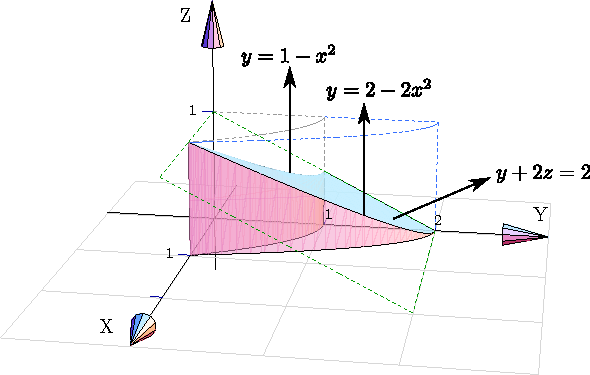
\includegraphics[width=2cm]{images/exersolido21}}
	& Solido $Q$ limitado por las superficies $y = 2 - 2 x^2;$ $y = 1 - x^2; \;\; y + 2 z = 2; \;\; x = 0$ y $z = 0;$ en el I octante.\\
\end{tabular}
\end{document}